\usetikzlibrary{calc}
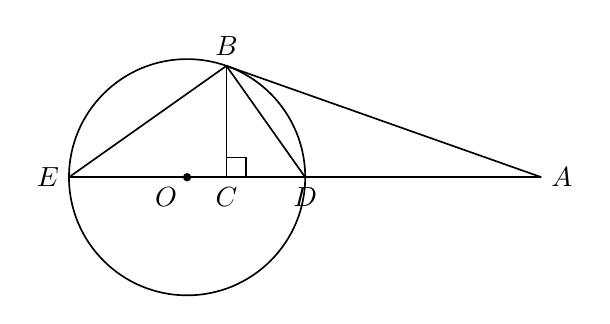
\begin{tikzpicture}[x=1cm,y=1cm,line width=.6pt,font=\normalsize]
\coordinate (O) at (0,0);
\coordinate (E) at (-1.5,0);
\coordinate (C) at (0.5,0);
\coordinate (D) at (1.5,0);
\coordinate (A) at (4.5,0);
\coordinate (B) at (0.5,1.41421);
\draw (O) circle[radius=1.5cm];
\draw (E)--(A);
\draw (B)--(C);
\draw (E)--(B);
\draw (B)--(D);
\draw (A)--(B);
\draw (0.5,0.25)--(0.75,0.25)--(0.75,0);
\fill (O) circle (1.5pt);
\node[left] at (E) {$E$};
\node[below left] at (O) {$O$};
\node[below] at (C) {$C$};
\node[below] at (D) {$D$};
\node[right] at (A) {$A$};
\node[above] at (B) {$B$};
\end{tikzpicture}
